\documentclass[11pt, a4paper, twoside]{article}   	% use "amsart" instead of "article" for AMSLaTeX format

\usepackage{geometry}                		% See geometry.pdf to learn the layout options. There are lots.
\usepackage{pdfpages}
\usepackage{caption}
\usepackage{minted}
\usepackage[german]{babel}			% this end the next are needed for german umlaute
\usepackage[utf8]{inputenc}
\usepackage{color}
\usepackage{graphicx}
\usepackage{titlesec}
\usepackage{fancyhdr}
\usepackage{lastpage}
\usepackage{hyperref}
\usepackage[autostyle=false, style=english]{csquotes}
\usepackage{mathtools}
\usepackage{tabularx}
\usepackage{varwidth}
\usepackage{mwe}
% http://www.artofproblemsolving.com/wiki/index.php/LaTeX:Symbols#Operators
% =============================================
% Layout & Colors
% =============================================
\geometry{
   a4paper,
   total={210mm,297mm},
   left=20mm,
   right=20mm,
   top=20mm,
   bottom=30mm
 }	

\definecolor{myred}{rgb}{0.8,0,0}
\definecolor{mygreen}{rgb}{0,0.6,0}
\definecolor{mygray}{rgb}{0.5,0.5,0.5}
\definecolor{mymauve}{rgb}{0.58,0,0.82}

\setcounter{secnumdepth}{4}


% the default java directory structure and the main packages
\newcommand{\imageDir}{../../images}
% =============================================
% Code Settings
% =============================================
\newenvironment{code}{\captionsetup{type=listing}}{}
\newmintedfile[javaFile]{java}{
	linenos=true, 
	frame=single, 
	breaklines=true, 
	tabsize=2,
	numbersep=5pt,
	xleftmargin=10pt,
	baselinestretch=1,
	fontsize=\footnotesize
}

\newmintedfile[csharpSourceFile]{csharp}{
	linenos=true, 
	frame=single, 
	breaklines=true, 
	tabsize=2,
	numbersep=5pt,
	xleftmargin=10pt,
	baselinestretch=1,
	fontsize=\footnotesize
}

\newmintedfile[xmlFile]{xml}{
	linenos=true, 
	frame=single, 
	breaklines=true, 
	tabsize=2,
	numbersep=5pt,
	xleftmargin=10pt,
	baselinestretch=1,
	fontsize=\footnotesize
}

\newmintedfile[cppSourceFile]{cpp}{
	linenos=true, 
	frame=single, 
	breaklines=true, 
	tabsize=2,
	numbersep=5pt,
	xleftmargin=10pt,
	baselinestretch=1,
	fontsize=\footnotesize
}

\newcommand{\xvdash}[1]{%
  \vdash^{\mkern-10mu\scriptscriptstyle\rule[-.9ex]{0pt}{0pt}#1}%
}

% =============================================
% Page Style, Footers & Headers, Title
% =============================================
\title{SVE - Projekt}
\author{Christoph Ruhsam, Marko Gattringer}

\lhead{SVE - Projekt}
\chead{}

\cfoot{}
\rfoot{ \thepage / \pageref{LastPage} }
\renewcommand{\footrulewidth}{0.4pt}

\pagestyle{fancy}
\begin{document}
\setlength{\headheight}{15mm}

\section{Dokumentation - SVE - UE05 - Projekt}
Christoph Ruhsam, Gattringer Marko

\subsection{Kurzbeschreibung}
Als MUS-Projekt wird eine App zur erleichterten Parkplatzsuche entwickelt. Das Backend zu dieser 
Anwendung wird mit JavaEE und Thorntail realisiert. Es wird eine Microservice-Architektur gewählt. 
Weiters werden Swagger (REST-Schnittstellendefinition) und Jaeger (Tracing über Serviceaufrufe) eingebaut. 
Die Services, sowie SwaggerUI und JaegerUI, laufen in OpenShift und können mittels Fabric8 einfach deployt werden. 
Die Build-, Test- und Deploymentvorgänge werden mithilfe von Openshift-Pipelines und Jenkins automatisiert. 
Arquillian wird als Testframework verwendet.

\subsection{Ziel / erwartetes Ergebnis}
Microservice-Architektur, welche Lokal (zu Test- und Entwicklungszwecken) als auch in Openshift lauffähig ist. 
Im optimalen Fall erkennt ein Client nicht, mit welcher Sprache/Technologie ein von ihm verwendetes Service implementiert ist.
Das heißt man ist nicht mehr an eine Implementierungssprache gebunden, sondern kann für die jeweilige Aufgabe die beste 
Sprache/Technologie auswählen (in diesem Fall Python für das MachineLearning-Service).

Es steht eine Infrastruktur zur Verfügung, mit der automatisierte Tests entwickelt werden können (Arquillian).
Es soll einfach möglich sein, einen Serviceaufruf (auch über mehrere Services hinweg) zu tracen (Jaeger).
Die Build-, Test- und Deploymentvorgänge werden mithilfe von Openshift-Pipelines und Jenkins automatisiert.


\subsection{Projektstruktur}
\begin{itemize}
	\item \textbf{ParkingManagerCoordinateService} (Java, Marko): Liest Koordinaten und weitere Informationen von Parkplätzen, Liefert zur aktuellen Position den nähesten freien Parkplatz
	\item \textbf{ParkingManagerParkingService}:(Java, Marko): Speichert neue Parkplätze, welche zum System hinzugefügt werden sollen, Liefert alle bereits gespeicherten Parkplätze
	\item \textbf{ParkingManagerAnalyzerService}: (Python, Marko): Nimmt eine Url einer Webcam entgegen und liefert die aktuelle Parkplatzsituation
	\item \textbf{project-stages.yml}: Bei jedem Microservice in src/main/resources zu finden. Hier können für die unterschiedlichen 
	Stadien der Entwicklung (zBsp.: Lokal, Openshift, ...) unterschiedliche Konfigurationen hinterlegt werden. So wird in unserem 
	Fall zBsp.: der Endpunkt des Jaeger-Agents konfiguriert. Dieser wird lokal als einfacher Dockercontainer gestartet und 
	ist unter \textbf{localhost:6832} zu erreichen. In Openshift wird dazu ein eigener Pod gestartet und kann dort unter \textbf{jaeger-agent:5775} erreicht werden.
	\item \textbf{maven-pipeline.yaml}: Definiert eine Openshift Pipeline, welche \\
	* den aktuellen Sourecode auscheckt\\
	* das jeweilige Service neu baut\\
	* alle Testfälle ausführt\\
	* ein neues Dockerimage erzeugt und in der Registry ablegt\\
	* das Service neu deployed\\
	* eine "Readiness"- und "Liveness"-Probe durchführt
\end{itemize}

\subsection{Architektur}
Folgende Abbildung zeigt die Architektur, wie die Infrastruktur am lokalen Entwicklerrechner aussieht (hier ist Openshift nocht nicht invoviert):
\begin{figure}[h]
	\centering
	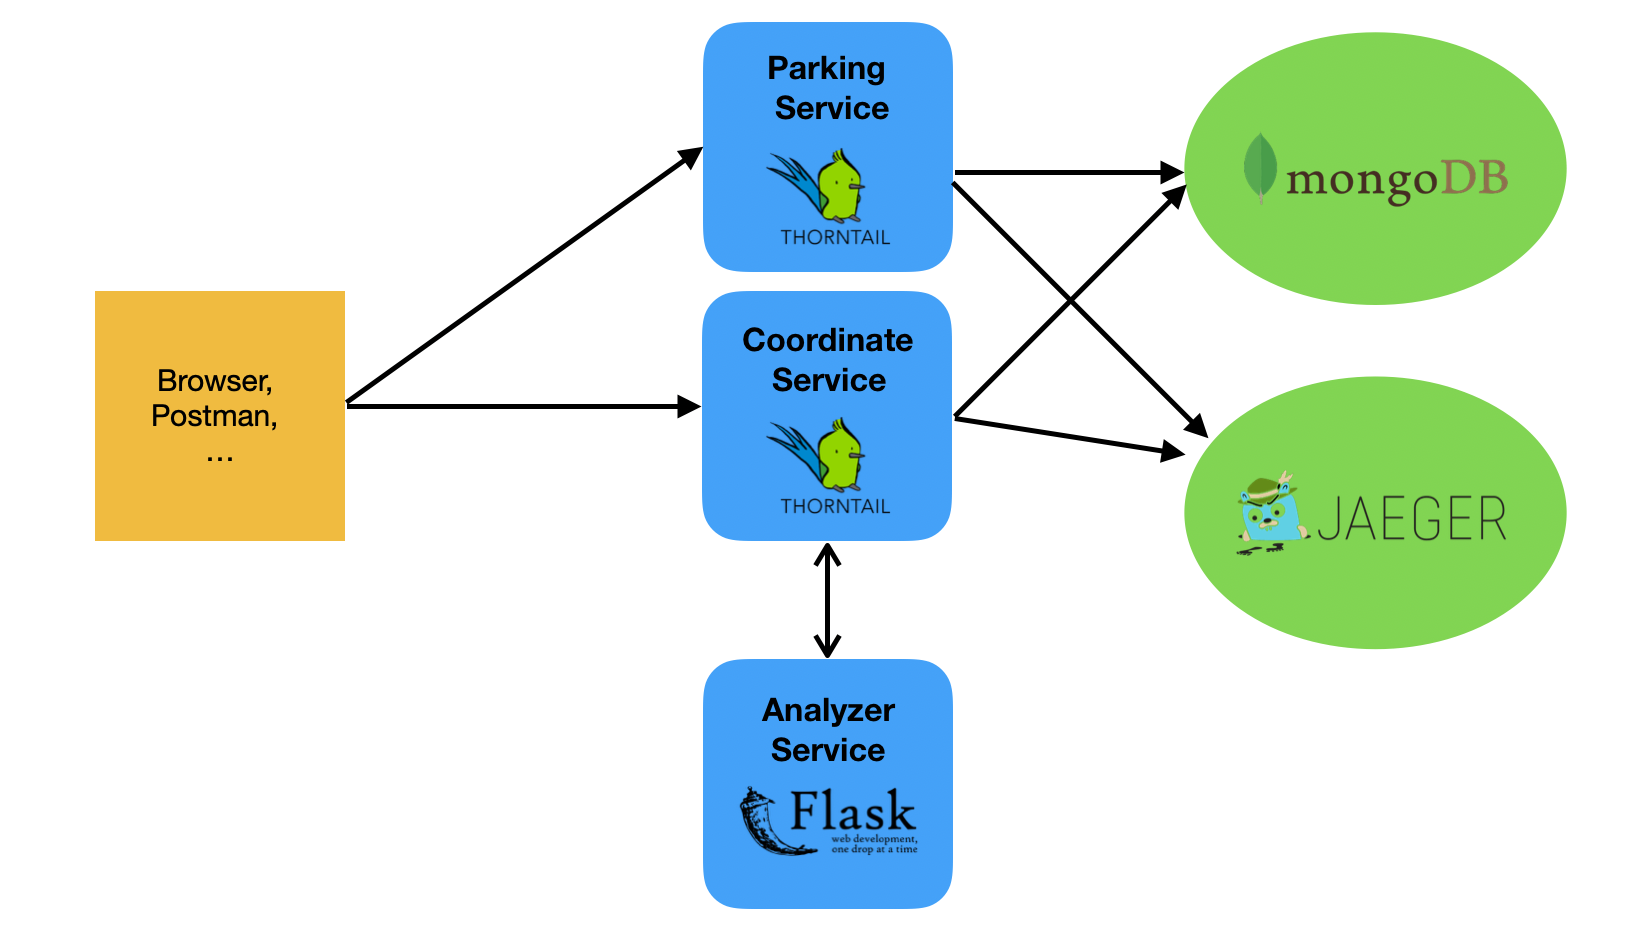
\includegraphics[scale=0.4]{\imageDir/architecture_local.png}
	\caption{Lokale Architekturskizze, alle Services können unabhängig voneinander gestartet werden.}
\end{figure}

In OpenShift sieht die Architektur wie folgt aus:
\begin{figure}[h]
	\centering
	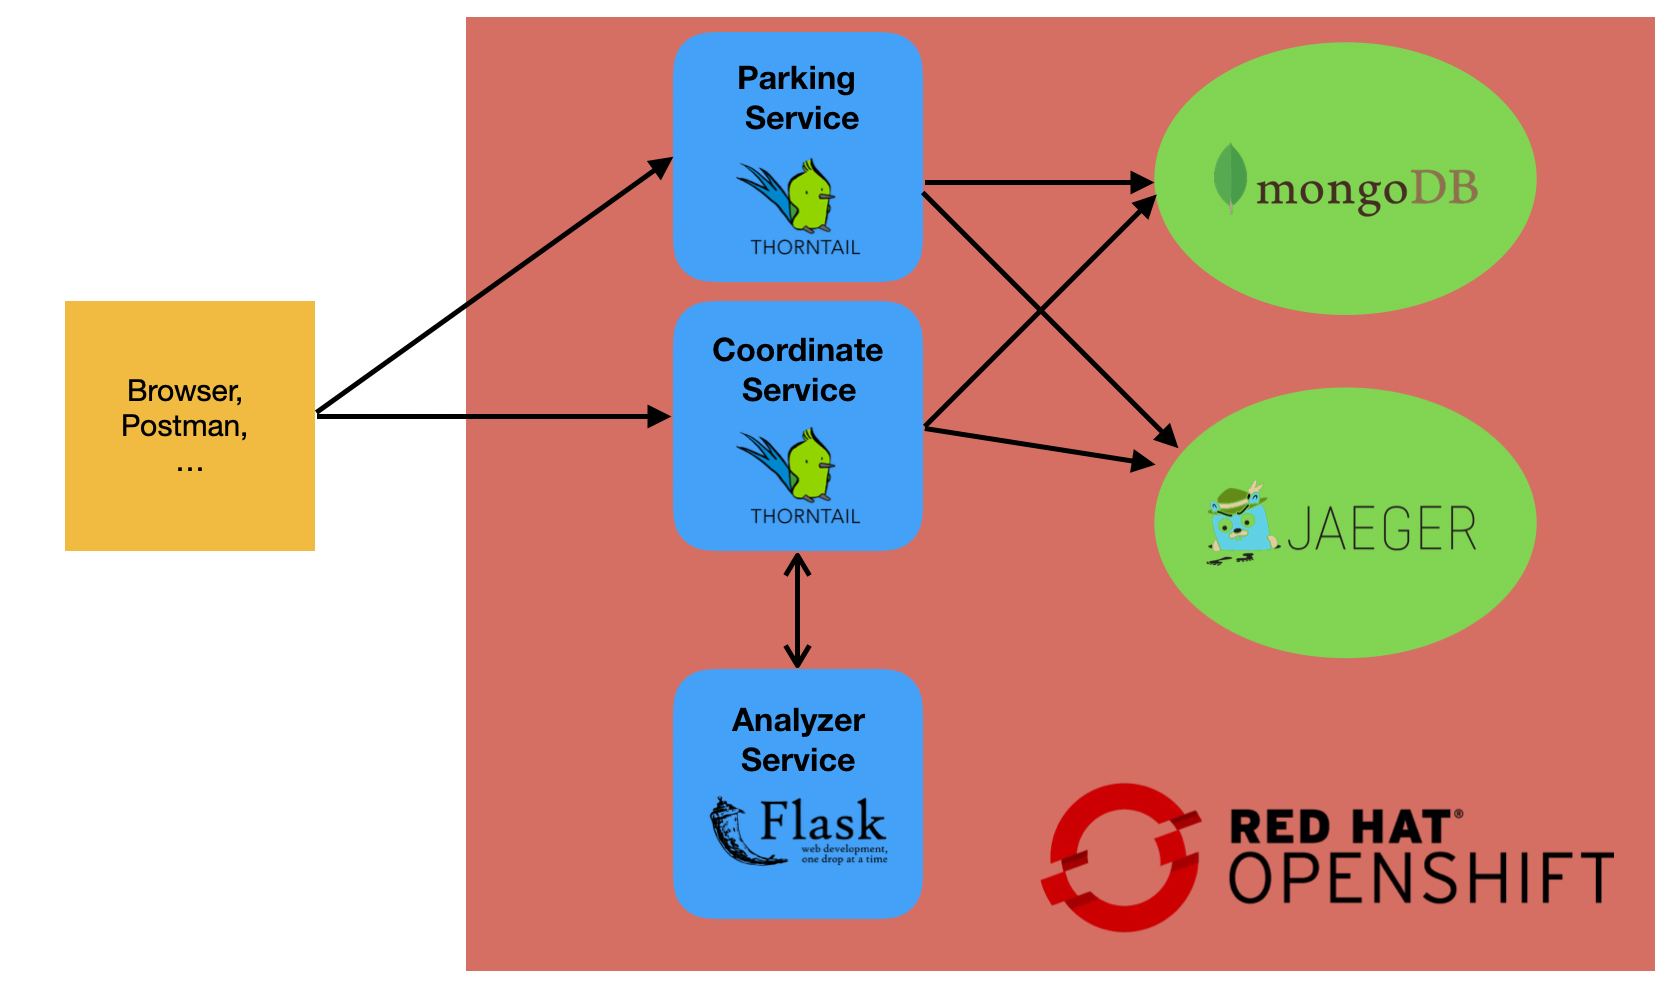
\includegraphics[scale=0.4]{\imageDir/architecture_openshift.png}
	\caption{Openshift Architekturskizze}
\end{figure}

\subsubsection{Verwendete Technologien/Bibliotheken}
\begin{itemize}
	\item \textbf{https://microprofile.io/:} Eine Initiative um Java EE für Microsservice-Architekturen zu optimieren.
	\item \textbf{https://www.jaegertracing.io/:} Ein Framework zum Monitoren von Microservices.
	\item \textbf{https://www.openshift.com/:} Ist eine Container-Plattform von Redhat, welche auf Docker und Kubernetes aufbaut.
	\item \textbf{http://arquillian.org/:} Ist eine Testframework, welches beim Testen von Java-Enterprise-Anwendungen unterstützt. 
	\item \textbf{http://fabric8.io/:} Hier wird das Maven-Plugin verwendet. Fabric8 vereinfacht und automatisiert das Deployment in OpenShift.
	\item \textbf{https://jenkins.io/:} Automation Server für automatisierte Build-, Test- und Deploymentvorgänge.
	\item \textbf{https://microprofile.io/} Unterschiedliche Metriken, wie Health, Count, Timed, ... 
\end{itemize}

\subsection{Setup}
\begin{enumerate}
	\item Gewünschte Release von https://github.com/openshift/origin/releases/ herunterladen 
	(ACHTUNG: bei 3.10 u. 3.11 gibt es aktuell Probleme beim erstellen von Volumes, mit 3.7 sollte es ohne Probleme funktionieren)
	\item In gewünschtes Verzeichnis entpacken und PATH Variable um dieses Verzeichnis erweitern
	\item Docker starten (muss laufen damit Openshift Cluster gestartet werden kann, basiert auf Docker-Images)
	\item \textbf{oc cluster up}: startet einen neuen Cluster
	\item \textbf{oc login}: am lokalen Cluster anmelden (fabric8 deployed in den Cluster an dem man aktuell eingeloggt ist) $\rightarrow$ USER/PASSWORT kann beliebig gewählt werden
	\item \textbf{oc new-project [PROJEKTNAME]}: Legt ein neues Projekt an
	\item \textbf{oc process -f https://raw.githubusercontent.com/jaegertracing/jaeger-openshift/master/all-in-one/jaeger-all-in-one-template.yml | oc create -f}: Deployt ein vorgefertigtes Jaeger Template
	\item \textbf{oc process -f https://raw.githubusercontent.com/sabre1041/openshift-api-swagger/master/openshift-api-swagger-template.yml | oc apply -f}: Deployt ein vorgefertigtes SwaggerUI Template
	\item \textbf{mvn fabric8:deploy -Pfabric8}: Muss in dem Root-Verzeichnis des jeweiligen Services ausgeführt werden. Deployt das Service in OpenShift.
\end{enumerate}

\subsection{OpenShift (beide)}
OpenShift ist eine OpenSource Container Application Platform und setzt auf Kubernetes auf.
Nach dem Befehl \textbf{oc cluster up} kann unter localhost:8443 die grafische Oberfläche aufgerufen werden.
Sind bereits Services in OpenShift deployt, sieht dies wie folgt aus:
\begin{figure}[h]
	\centering
	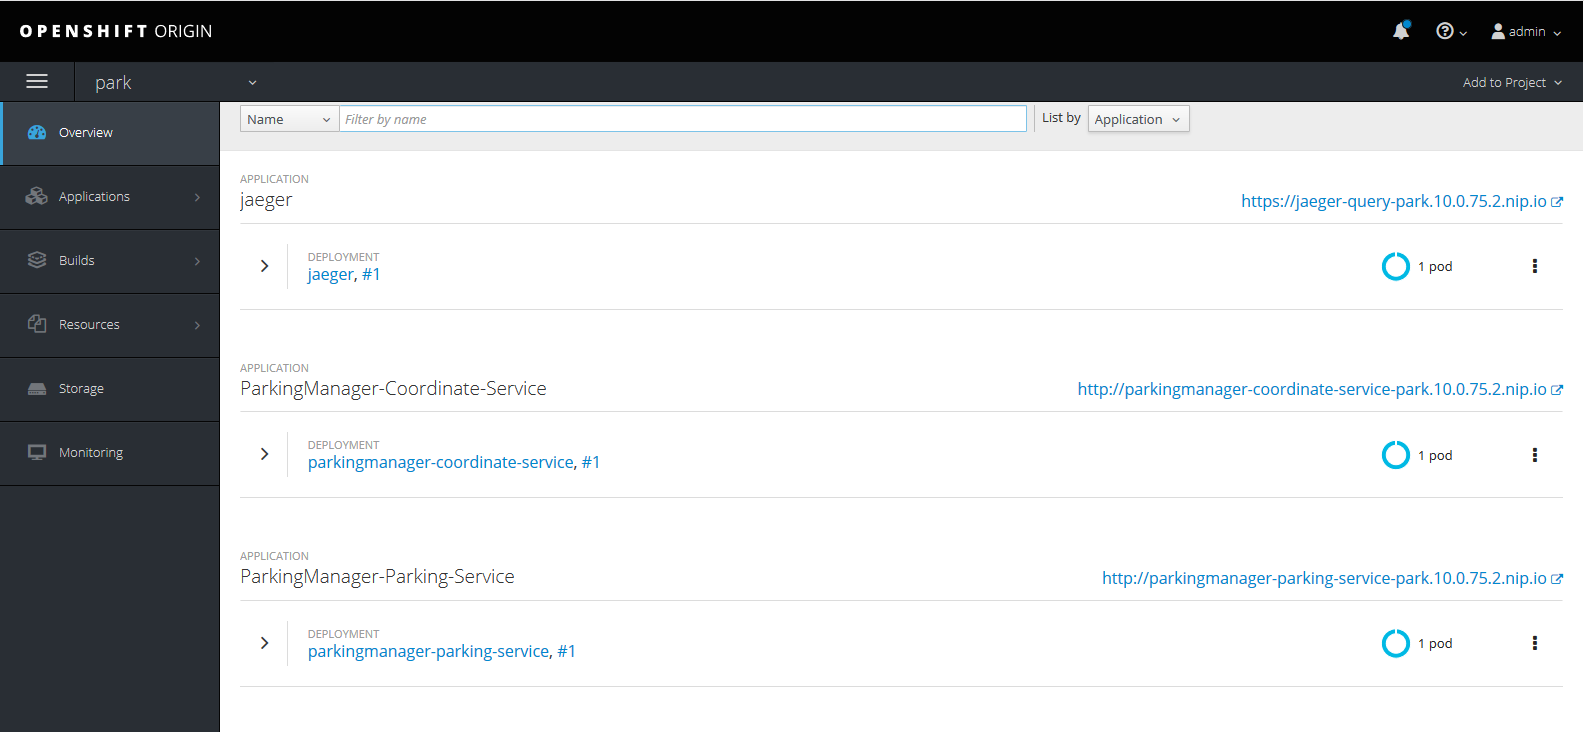
\includegraphics[scale=0.4]{\imageDir/openshift-view.png}
	\caption{OpenShift Service View}
\end{figure}

Ein Service kann auf hinauf-/heruntergescaled werden. Dadurch können mehrere Pods gestartet werden. Das Load-Balancing wird von OpenShift übernommen.
\begin{figure}[h]
	\centering
	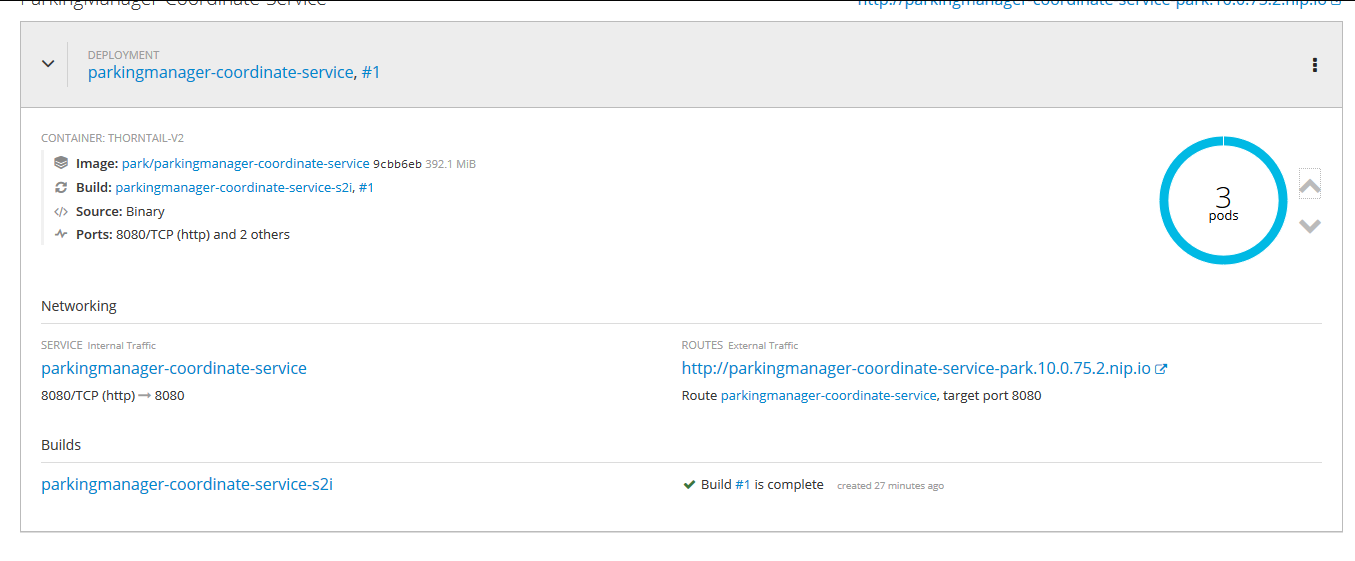
\includegraphics[scale=0.4]{\imageDir/openshift-scaledup.png}
	\caption{OpenShift Scaled Up}
\end{figure}

\newpage
\subsection{OpenTracing mit Jaeger (Christoph)}
Jaeger ist ein Tracing System, das OpenSource zur Verfügung steht. Es wird für Monitoring und Troubleshooting bei Microservice-Architekturen verwendet.
Um Jaeger mit Thorntail und JavaEE verwenden zu können, werden folgende Teile benötigt:
\begin{itemize}
	\item io.thorntail.jaeger und io.thorntail.microprofile-opentracing Dependencies
	\item Annotation **@Traced** bei der REST-Resource
	\begin{itemize}
		\item @Traced kann über der Klasse angegeben werden -- alle Methoden der Klasse werden getraced
		\item @Traced kann aber auch nur über einzelnen Methoden angegeben werden. Es werden lediglich diese Methoden getraced.
	\end{itemize}
	\item Im *project-stages.yml* folgende Konfigurationsparameter:
	\begin{itemize}
		\item service-name: Service Name der mit den Spans assoziiert wird
		\item agent-host: Host unter dem der jaeger-agent erreichbar ist
		\begin{itemize}
			\item Dieser ist für die lokale Entwicklung localhost
			\item Und in OpenShift **NICHT** die Route von Jaeger, sondern der Container Name von Jaeger. In unserem Fall "jaeger-agent".
		\end{itemize}
		\item agent-port: Port unter dem der jaeger-agent erreichbar ist.
		\item reporter-flush-interval: Definiert, wie oft Jaeger die Spans flusht
		\item sampler-type: Definiert den Typ des Samplers, z.B.: probabilistic oder const
		\item sampler-parameter: Configurations-Wert für den Sampler, z.B.: probabilistic = 0.001
	\end{itemize}
\end{itemize}

Ist Jaeger und ein Service deployed und eine getracte REST-Resource dieses Service wird aufgerufen, wird der Span an Jaeger gesendet. Mittels der JaegerUI, deren URL in OpenShift zu sehen ist, können die Traces angesehen werden.

\begin{figure}[h]
	\centering
	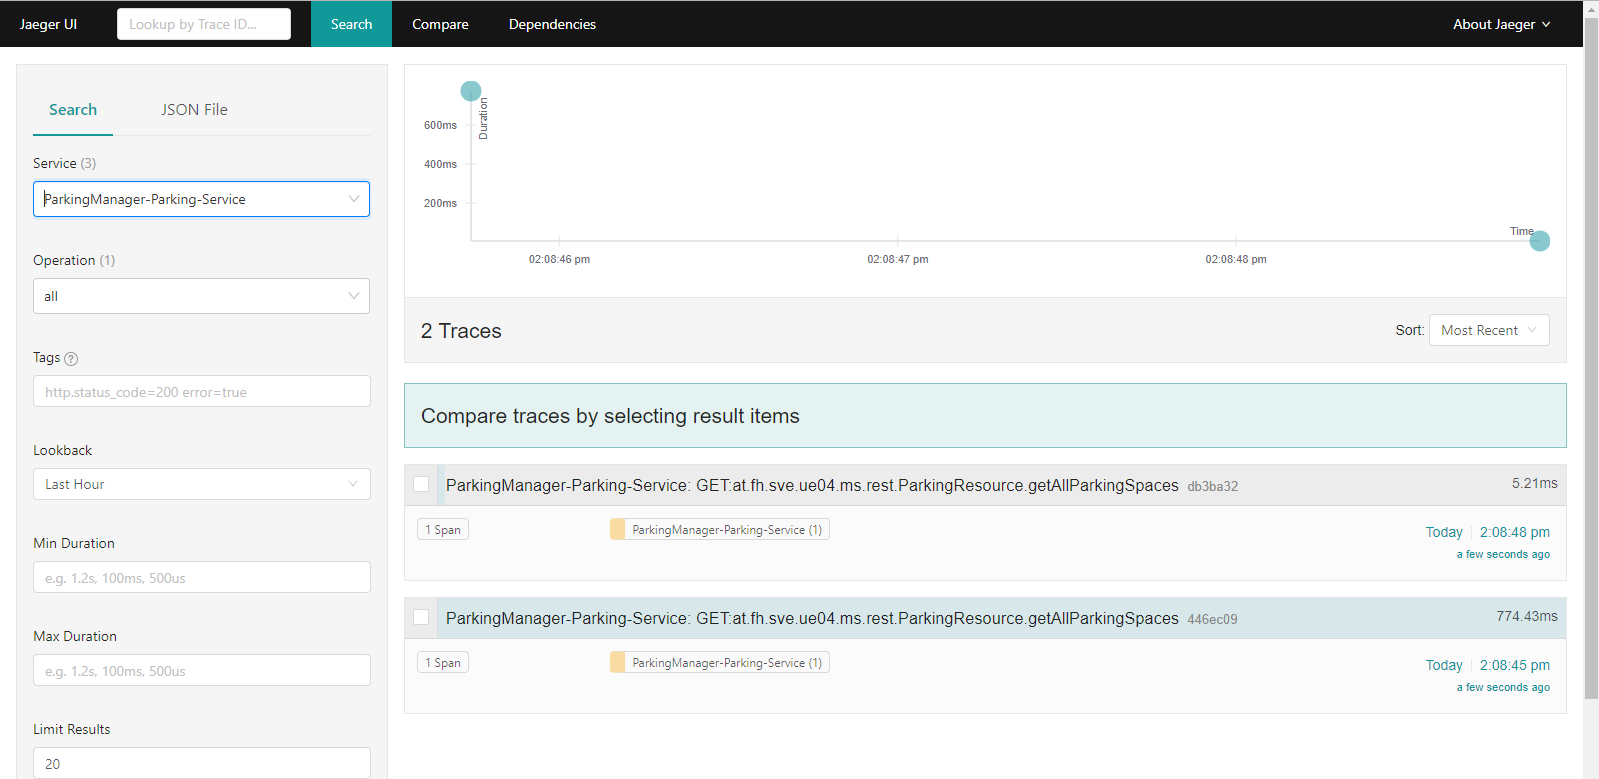
\includegraphics{\imageDir/jaeger_ui.png}
	\caption{JaegerUI}
\end{figure}

Im project-stages.yml befinden sich 2 verschiedene Stages. Die Stage \textbf{test} zum lokalen Deployment und die Stage \textbf{openshift} für das Deployment in OpenShift.
Um eine Stage auszuwählen, muss beim Deployment der Maven-Parameter \textbf{-Dswarm.project.stage=[stage]} mitgegeben werden.
Default ist die Stage openshift eingestellt.

\subsection{MongoDB (Marko)}
in $\backslash$etc$\backslash$docker$\backslash$MongoDB findet sich ein Dockerfile, welches beim Hochfahren die benötigte Datenbank 
erzeugt mit mit Daten befüllt. Das hier erzeugte Image kann sowohl lokal als auch in Openshift genutzt 
werden.

Zum einfacheren Testen wurde für das Service \textbf{ParkingManagerCoordinateService} ein Mock-Service 
implementiert, welches mittels einer CDI-Alternative, die im beans.xml definiert wird, aktiviert oder 
deaktiviert wird. Dieses Mock-Service kommt auch bei den Unit-Tests zum Einsatz.

\subsection{Arquillian (Marko)}
Arquillian ist ein Framework, welches beim Entwickeln von Unit-Tests für Jave-Enterprise-Anwendungen unterstützt. Arquillian liefert 
einen eigenen Runner mit, welcher mit der Annotation \textbf{@org.junit.runner.RunWith} verwendet wird. Dieser Runner verlangt 
eine Methode innerhalb des Testfalles, welche mit \textbf{org.jboss.arquillian.container.test.api.Deployment} annotiert ist. 
In dieser Methode wird das Deployment für den aktuellen Test zusammengebaut. Das bedeuted, man kann in jedem Testfall festlegen welche 
Komponenten und Klassen deployed und getestet werden. Ein weiterer Vorteil dieser Vorgehensweise ist, dass man in jedem Test ein angepasstes 
beans.xml verwenden kann, in welchem dann zBsp. Alternativen aktiviert werden, welche externe Serviceaufrufe oder DB-Zugriffe mocken.

\subsection{REST (beide)}
Die beiden Service \textbf{ParkingManagerCoordinateService} und \textbf{ParkingManagerParkingService} stellen die REST-Schnittstellen für den Python-Client und den Angular-Client bereit.
Das Service \textbf{ParkingManagerCoordinateService} dient zum Lesen der Koordinaten und wird vom Angular-Client verwendet.
Das Service \textbf{ParkingManagerParkingService} dient zum Schreiben und Aktualisieren der Label-Daten und wird vom Python-Client verwendet.
Beide Services implementieren einen CorsResponseFilter, damit die Clients keine Probleme mit CORS haben.
Beide Services kommunizieren mit der MongoDB mittels HibernateOGM.

\subsection{REST-Dokumentation mit Swagger (Christoph)}
Die REST-Dokumentation wird mittels Swagger-erstellt. Dazu werden die beiden Dependencies \enquote{swagger-annotations} und \enquote{swagger-jaxrs} benötigt. Mittels den Annotationen \textbf{@Api} über der Resource-Klasse und \textbf{@Api-Operation} über den REST-Methoden, erstellt Swagger ein Swagger.json in dem die REST-Dokumentation enthalten ist.
Im Package \textbf{config} befindet sich auch eine SwaggerConfig, mit dem auch eine Version, Author und ein Kontakt gesetzt werden.

Die Swagger-UI läuft in OpenShift. In dieser kann das swagger.json eines Service aufgerufen und somit die REST-Schnittstelle einfach getestet werden.
z.b.: <service-url>$\backslash$api$\backslash$swagger.json

\subsection{Jenkins (Marko)}
Jenkins ist ein webbasierter Buildserver, der es möglich macht eine Software vollautomatisiert zu bauen, zu 
testen und zu deployen. 

In diesem Projekt wird ein Jekins auch gleich in Openshift betrieben. Einziger Unterschied zu einem \enquote{normalen}
Jenkins auf irgendeinem Server ist, dass in Openshift ein Jenkins-Master als Pod deployed wird und die einzelnen 
Jobs als Openshift-Pipelines angelegt werden. Dieser Ansatz ermöglicht es, den \enquote{einfachen} Jenkinsbuild um einige 
Funktionen zu erweitern (erzeugen und ablegen von DockerImages in der Openshift-Registry, Openshift-Befehle können 
einfach aufgerufen werden, ...). 

Die hier gebauten Pipelines beschreiben folgende Schritte:
\begin{itemize}
	\item  Pullen der neuen Sourcen des jeweiligen Services
	\item Bauen des jeweiligen Services
	\item Ausführen der Testfälle
	\item Erzeugen eines neuen Dockerimages und ablegen in der Dockerregistry von Openshift
	\item Deployen der neuen Version
	\item Testen ob Deployment gut gegangen ist
	\item Laufende Prüfung, ob das Service noch lebt
\end{itemize}


\subsection{Metrics (Christoph)}
Auch Metriken werden bereitgestellt und können bei jedem Service unter der URL $<$service$>$/metrics/application abgefragt werden.
Es werden dabei die Metriken \textbf{Count}, \textbf{Timed} und \textbf{Health} bereitgestellt.
\begin{itemize}
	\item \textbf{Count: }Zählt, wie oft eine Ressource aufgerufen wurde.
	\item \textbf{Timed: }Berechnet den Mittelwert der Dauer von Request bis Response aller Anfragen pro Ressource.
	\item \textbf{Health: }Gibt Auskunft über das Befinden eines Pods.
\end{itemize}

\end{document}
